\chapter{Introduction and Literature Review} % Chapter Title
\label{LR}

\section{The atmosphere}
\label{LR:Atmos}
  % Overarching description of atmosphere
  The atmosphere is made up of various gases held to the earths surface by gravity. 
  These gases undergo transport on all scales, from barbeque smoke being blown into your face to smoke plumes from forest fires travelling accross the world and depositing in the antarctic snow.
  They take part in various chemical reactions along the way, largely driven by solar input and interactions with eachother.
  Various chemicals are lofted into the atmosphere by soil, trees, factories, cars, seas and oceans, you name it.
  They are also deposited back to the surface both directly and in rain drops.
  
  % Air
  Mostly the atmosphere is made up of nitrogen (N$_2$: $\sim 78\%$), oxygen (O$_2$: $\sim 21\%$), and argon (Ar: $\sim 1\%$).
  Water (H$_2$O) ranges from $0.001$ to $1\%$ depending on evaporation and precipitation.
  Beyond these major constituents the atmosphere has a vast number of \textit{trace gases}, including carbon dioxide (CO$_2$: $\sim 0.4\%$), Ozone (O$_3$: $.000001$ to $0.001\%$), and methane (CH$_4$: $\sim 0.4\%$) \cite[][Ch. 2]{BrasseurJacob2017}.
  Trace gases in the atmosphere can have a large impact on living conditions.
  They react in complex ways with other elements (anthropogenic and natural), affecting various ecosystems upon which life depends.
  
  % TODO: Pressure
  Most of the atmosphere ($\sim 85\%$) is within 10~km of the earths surface.
  This is due to air pressure, which decreases logarithmically with altitude.
  

  % TODO: Structure lead in
  
  \subsection{Structure}
  \label{LR:Atmos:Struct}
    
    % TODO: Boundary layer
    
    % TODO: Troposphere
    
    % TODO: Stratosphere
    
  % Chemistry
  \subsection{Chemistry}
  \label{LR:Atmos:Chem}
    % Oxidation and Radicals
    \subsubsection{Hydroxyl radicals}
    The OH radical drives many processes in the atmosphere, especially during the day when photolysis of ozone drives OH concentrations \citep{Atkinson2000}.    
    OH is a key species which reacts with nearly all the organic compounds in the troposphere.
    The exceptions are chlorofluorocarbons (CFCs), and Halons not containing H atoms \citep{Atkinson2000}.
    OH and HO$_2$ concentrations largely determine the oxidative capacity of the atmosphere.
    Oxidation and photolysis are the two main processes through which VOCs are broken down into HCHO, O$_3$, CO$_2$ and various other species.
    Over land, isoprene (C$_5$H$_8$) and monoterpenes (C$_10$H$_16$) account for 50\% and 30\% of the OH reactivity respectively \citep{Fuentes2000}.
    
    In the late 90's it was thought that OH radicals are formed exclusively from photolysis of O$_3$, HONO, HCHO, and other carbonyls (R$_2$C=O) \cite{Atkinson2000}.
    Isoprene (C$_5$H$_8$) was thought to be a sink of OH until it was shown by \cite{Paulot2009b} that the radicals are recycled.
    This recycling process is discussed in more detail in section \ref{LR:VOCs:IsopCascade}.
    
    Ozone is an important precursor to HO, as excited oxygen atoms (O(${}^1$D) are created through photolysis, which then go on to mix with water and form OH, as shown in this equation taken from \cite{Atkinson2000}:
    \begin{equation}
    \begin{aligned}
    O_3 + \text{hv}         & \to  O_2 + O({}^1D)   && (\lambda \le 335 \text{nm}) \\%
    O({}^1D) + M            & \to  O({}^3P) + M     && (M=N_2, O_2)               \\%
    O({}^3P) + O_2 + M      & \to  O_3 + M          && (M=\text{air})             \\%
    O({}^1D) + H_2O         & \to  2OH              &&                            \\%
    \end{aligned}
    \label{LR:Radicals:eqn_O3toOH}
    \end{equation}
    This shows how some of the O$({}^1D)$ recycles back to Ozone, while some forms OH.
    NB: The wavelength was updated to 350~nm in \cite{AtkinsonArey2003}.
    
    % Photolysis stuff
    Ozone is also a very important substance for formation of radicals (NO$_3$, OH) in the troposphere through photolysis in the presence of water.
    
    \subsubsection{Nitrate radicals}
    Nitrate radicals NO$_3$ are largely formed through ozone reactions.
    They are photolysed very rapidly during they day, with a lifetime of about 5~s \citep{Atkinson2000}.
    If NO and O$_3$ are both in the atmosphere, the following reactions \citep{Atkinson2000} occur:
    \begin{equation}
    \begin{aligned}
    NO + O_3         & \to NO_2 + O_2      && \\%
    NO_2 + O_3       & \to NO_3 + O_2      && \\%
    NO_3 + \text{hv} & \to NO + O_2        && (\sim 10\%)  \\%
    NO_3 + \text{hv} & \to NO_2 + O({}^3P) && (\sim 90\%)  \\%
    \end{aligned}
    \label{LR:Radicals:eqn_O3toNO2}
    \end{equation}
    A build up of NO$_3$ radicals can be seen at night, when photolysis is not removing them quickly \citep{Atkinson2000,Brown2009}.
    
    Since radicals play such a big role in regulating many chemical reactions in the atmosphere it's important for models to accurately represent them (eg. \cite{Travis2014}). 
    This is difficult as they are coupled with so many other species and measurements of OH are not readily available on a global scale.
    
    
    % Ozone lead in
    Ozone in the lower atmosphere is a serious hazard that causes health problems \citep{Hsieh2013}, damages agricultural crops worth billions of dollars \citep{Avnery2011,Yue2017}, and increases the rate of climate warming \citep{IPCC_2013_chap8}.

\section{Ozone}
\label{LR:O3}
  %TODO What is ozone
  Ozone (O$_3$) is mostly located in the stratosphere, where it helpfully prevents much of the shorter wave length solar radiation from reaching the earth's surface (ie UV light).
  However around 11\% of the total column of ozone is located in the troposphere (TODO: cite), where it has several deleterious effects.
  Around 5 to 20 percent of all air pollution related deaths are due to ozone (\cite{Monks2015}).
  In the short term, ozone concentrations of $\sim$50-60~ppbv over eight hours or $\sim$80~ppbv over one hour are agreed to constitude a human health hazard \citep{Ayers2006,Lelieveld2009}. 
  Long term exposure to lower levels cause problems with crop loss and ecosystem damage \citep{Emberson2003}, and both short and long term concentrations may get worse in the future \citep{Lelieveld2009, Stevenson2013}.
  Further tropospheric ozone enhancements are projected to drive reductions in global crop yields equivalent to losses of up to \$USD$_{2000}$ 35 billion per year by 2030 \citep{Avnery2011}, along with detrimental health outcomes equivalent to $\sim$\$USD$_{2000}$11.8 billion per year by 2050 \citep{Selin2009}.
  Recently \cite{Yue2017} showed that the net effect of near-surface ozone on is a $\sim 14\%$ decrease in net primary productivity (NPP) in China, which could be reduced by $\sim 70\%$ with drastic measures by 2030.
  
  %Structure of ozone layer chapman eqn etc.
  In the stratosphere ozone production is generally driven by the Chapman mechanism, as high energy light (with wavelengths $\lambda<242$~nm) photolyses the molecular oxygen (O$_2$) in the atmosphere \citep[][Chapter 3, section 2]{BrasseurJacob2017}.
  The Chapman mechanism involves several equations which lead to rough equilibrium of O, O$_2$, O$_3$ and pressure, as follows:
  \begin{eqnarray*}
    \label{LR:O3:eqn_Chapman}
    \textrm{O}_2 + hv(\lambda < 242 \text{nm}) & \rightarrow & \text{O} + \text{O} \\
    \text{O} + \text{O}_2 + \text{M} & \rightarrow & \text{O}_3 + \text{M} \\
    \text{O}_3 + hv(\lambda < 1180 \text{nm}) & \rightarrow & \text{O} + \text{O}_2 \\
    \text{O} + \text{O}_3 & \rightarrow & \text{O}_2 + \text{O}_2 \\
  \end{eqnarray*}
  Where $hv$ represents radiation and M is an inert molecule (such as N$_2$).
  The high energy photons ($\lambda < 242$~nm) are present from the top of the atmosphere but are mostly removed before reaching the troposphere.
  The lifetime of O against loss by O$_2$ is less than a second in the troposphere, and produced O$_3$ quickly returns to O and O$_2$, as low energy ($\lambda < 1180$~nm) light and M are abundant.
  The gradient of light penetration in addition to the logarithmic decrease in atmospheric pressure (which affects M abundance) drives (using the Chapman equation) the vertical profile of ozone into what is called the ozone layer, where most of the ozone is in the stratosphere.
  This mechanism requires radiation so only takes place during the daytime, during the night there are different processes driving ozone chemistry.
  
  % TODO things that affect ozone concentrations 
  Smoke plumes from biomass burning can carry ozone precursors, creating higher ozone concentrations downwind of the plume's source.
  Fire emissions include a range of chemicals and each year the affects of fire or burning seasons blanket the northern and southern hemispheres independently.
  
  TODO: get access to Hegglin (\url{10.1038/ngeo604}) \citep{Hegglin2009}
  
  % Measurements
  Since the Montreal Protocol on Substances that Deplete the Ozone Layer was established in August 1987, and ratified in August 1989, several satellites and many measurement stations were set up to monitor ozone in the stratosphere.
  However, in the southern hemisphere there are relatively few records of ozone (\cite{Huang2017}).
  One method of measuring ozone in the troposphere and stratosphere is by releasing weather balloons (with attached ozone detectors) which take readings as they rise up to around 30~km, giving a vertical profile of concentrations.
  Since 1986, Lauder, New Zealand (45$^{\circ}$S, 170$^{\circ}$E) has released ozonesondes allowing a multi-decadal analysis of ozone concentrations over the city \citep{Brinksma2002}.
  Kerguelan Island (49.2$^{\circ}$S, 70.1$^{\circ}$E), also has a record of ozonesonde profiles, which are directly in the path of biomass burning smoke plumes transported off shore from Africa \citep{Baray2012}.
  SHADOZ is the southern hemispheric additional ozone project, which have released sondes from 15 sites at different times \url{http://tropo.gsfc.nasa.gov/shadoz/}.
  
  What drives ozone in the troposphere? Two main contributors are transport from the stratosphere and creation due to biogenic emissions of precursors. 
  At smaller (regional) scales anthropogenic emissions are also important, especially in large cities such as Sydney due to NO$_X$ emissions from traffic and power production.
  
  \subsection{Stratosphere to troposphere transport}
    \label{LR:O3:STT}
    %% STT
    Historically (in the late 1990's), ozone transported down from the stratosphere was thought to contribute 10-40~ppb to tropospheric ozone levels, matching tropospheric production \citep{Atkinson2000, Stohl2003}.
    This number was revised down over the years as measurement and modelling campaigns improved our understanding of global scale transport, mixing, and chemistry \citep{Monks2015}.
    Recently \cite{Kuang2017} analysed various measurements in south-east USA and observed STT influence which can be seen to affect surface ozone levels.
    In their work they use high spectral resolution lidar (HSRL), ozonesondes, ozone lidar, and airborn in-situ measurements give the structure and temporal evolution of ozone and the low front weather system.
    
    Ozone transported to the troposphere from the stratosphere can occur through diffusion (slow process (TODO: Cite)) or through mixing, often called Stratosphere to Troposphere Transport events (STT), or intrusions.
    TODO: compare these two processes and their impacts briefly.
    Recently global chemical transport models (CTMs) have been used to trace how much ozone is being transported to the troposphere from the stratosphere.
    There are a few methods of doing this, such as \cite{Ojha2016}, who use the ECHAM5 CTM with a tracer that keeps track of ozone formed and transported from the stratosphere.
    Model based estimates generally require validation against actual measurements, such as those from ozonesondes or satellites.
    %Hegglin, M. I., and T. G. Shepherd (2009), Large climate-induced changes in ultraviolet index and stratosphere-to-troposphere ozone flux, Nature Geosci, 2(10), 687 \selectlanguage{english}691, doi:10.1038/NGEO604.
    \cite{Hegglin2009} estimate that climate change will lead to increased STT due to an acceleration in the Brewer Dobson circulation.
    They estimate $\sim 30$, and $\sim 121$~Tg yr$^{-1}$ increases (relative to 1965) in the southern and northern hemispheres respectively
    
    \cite{Liu2017} examine southern hemispheric ozone and the processes which control its inter-annual variability (IAV).
    IAV is the standard deviation of ozone anomalies (difference from the monthly mean).
    They show that ozone transported from the stratosphere plays a major role in the upper troposphere, especially over the southern Indian ocean during austral winter.
    While stratospheric transport mostly impacts the upper troposphere, some areas are impacted right down to the surface.
    \cite{Liu2017} look at modelled tropospheric ozone sensitivity to changes in stratospheric ozone, ozone precursor emissions, and lightning over the southern hemisphere from 1992--2011. 
    Their work suggest ozone at 430~hPa is mostly stratospheric in September over 20$^{\circ}$S to 60$^{\circ}$S at all longitudes.
    They also see tropospheric ozone sensitivity to emissions from South America (0--20$^{\circ}$S, 72.5--37.5$^{\circ}$W), southern Africa (5--10$^{\circ}$S, 12-38$^{\circ}$E), and South to South-east Asia (70-125$^{\circ}$E, 10$^{\circ}$S--40$^{\circ}$N).
    In the USA recent work by \cite{Lin2015} suggests that intrusions during spring are increasing surface ozone levels.
    Their work also recommends that understanding of frequency and cause of STT needs to be improved to effectively implement air quality standards.
    
    %Lead in to chem production
    An analysis of the Atmospheric Chemistry and Climate Model Inter-comparison Project (ACCMIP) simulations by \cite{Young2013} found STT is responsible for $540\pm140$~Tg yr$^{-1}$, equivalent to $\sim$11\% of the tropospheric ozone column, with the remainder produced photochemically \citep{Monks2015}.
  
  \subsection{Chemical production}
    The tropospheric ozone concentrations rely on climate and ozone precursor emissions; including NO, NO$_2$, CO, VOCs, and HCHO \citep{Atkinson2000, Young2013, Marvin2017}. 
    Ozone predictions are uncertain and difficult due to the vagaries of changing climate which affects both transport, deposition, destruction, and plant based precursor emissions.
    All of these processes are tightly coupled and difficult to accurately model, as they depend on uncertain assumptions such as CO$_2$ dependency \citep{Young2013}.
    Even with all the work done in the prior decades there remains large uncertainties about ozone precursors in the troposphere \citep{Mazzuca2016}.
    
    %% How VOCs and Ozone interact:
    Ozone is formed in the troposphere through oxidation of VOCs in the presence of NO$_X$.
    VOCs are described in the following section (Section \ref{LR:VOCs}).
    Net formation or loss of O$_3$ is determined by interactions between VOCs, NO$_X$, and HO$_X$, and is a complicated system of positive and negative feedbacks \citep{Atkinson2000}.
    Figure \ref{LR:VOCs:fig_NOXVOCOzone} shows the non-linear affect of NO$_X$ and VOC concentrations on ozone production over Houston, as modelled in \cite{Mazzuca2016}.
    Recently the relationship has been examined on the intradiel timescale showing that ozone production can be more or less sensitive to VOCs at different hours depending on location various other factors \citep{Mazzuca2016}.
    
    \begin{figure}
      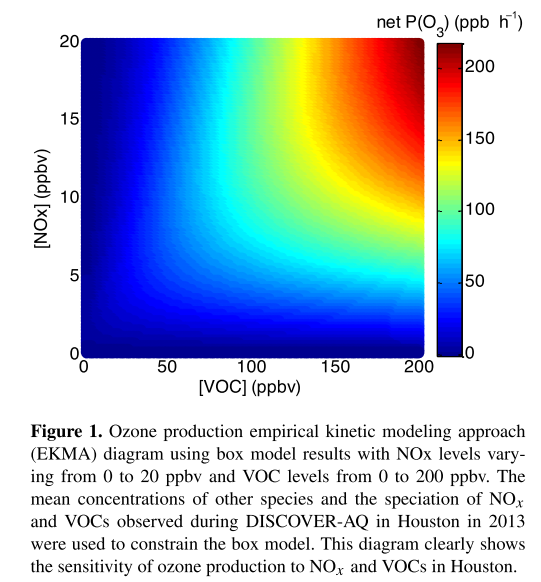
\includegraphics[width=.75\textwidth]{Figures/Mazzuca2016_NOxVOCOzone.png}
      \caption{Ozone production figure copied from \cite{Mazzuca2016}.}
      \label{LR:VOCs:fig_NOXVOCOzone}
    \end{figure}
    
    
    %TODO: formulae which regulate ozone levels 
    Ozone in rural areas is often higher than in populous cities, as the high NO levels titrate the O$_3$.
    Equation \ref{LR:Radicals:eqn_O3toNO2} shows how NO and O$_3$ lead to NO$_2$ and the very short lived NO$_3$ radical.
    
    % Loss pathways
    Tropospheric ozone is lost via chemical destruction and dry deposition, estimated to be $4700\pm700$ Tg yr$^{-1}$ and $1000\pm200$ Tg yr$^{-1}$, respectively \citep{Stevenson2006}.
    The main loss channel is through equation \ref{LR:Radicals:eqn_O3toOH}, where photolysis and pressure create OH from the O$_3$.
    

\section{VOCs}
\label{LR:VOCs}
  % What they are
  Organic compounds are members of a large class of chemicals whose molecules contain carbon, with the exception of a few compounds such as carbides, carbonates (CO$_3$), and simple oxides of carbon and cyanides.
  Organic compounds can be categorised based on their vapour pressure, which is the tendency of a liquid or solid to vaporise.
  Compounds with high vapour pressures at standard temperature are classed as volatile, and have a felicity to evaporate at low temperatures.
  Plants contain tens of thousands of organic compounds, it's likely that fewer than 40 are emitted due to the low volatility of most of them \citep{Guenther2000}.
  
  Atmospheric organic compounds are legion and differ by orders of magnitude with respect to their fundamental properties, such as volatility, reactivity, and cloud droplet formation propensity.
  Volatile organic compounds (VOCs) have vapour pressure greater than $10^{-5}$~atm, and are mostly generated naturally by plants, which emit around 1000\tgpyr \citep{Guenther1995, Glasius2016}.
  Due to their high volatility these compounds are generally seen in the gas phase.
  Organic compounds with a lower volatility are classed as semi-volatile (SVOCs: vapour pressure between $10^{-5}$ and $10^{-11}$~atm) are seen in both gas and particle phase depending on temperature and pressure.
  Organic compounds with even lower vapour pressure are generally found in the particle phase in aerosol particulate matter \citep{Glasius2016}.
  Understanding the drivers of trends in biogenic VOC emissions (BVOCs) is needed in order to estimate future carbon fluxes, changes in the water cycle, air quality, and other climate responses \citep{Yue2015}.
  

  %% What do VOCs do?
  VOCs are an important driver of atmospheric processes, especially near forests.
  VOC emissions result in radical cycling, acid deposition, production of tropospheric ozone, and secondary organic aerosols (SOAs) \citep{Atkinson2000, Kanakidou2005}.
  A regional-model study in Europe (\cite{Aksoyoglu2017}) has also shown VOCs impact secondary inorganic aerosol concentrations.
  These have impacts on climate (through radiative forcing) and air quality, affecting both human health and crop yields \citep{IPCC_Chapter2, Avnery2011, Lelieveld2015}.
  
  % voc sources
  The major source of VOCs in the atmosphere is biogenic, with around 90\% of emissions (globally) coming from natural sources \citep{Guenther1995,Guenther2006, Millet2006}.
  Global non-methane VOC (NMVOC) levels are estimated at 85~\%, 13~\%, and 3~\% from biogenic, anthropogenic, and pyrogenic sources respectively \citep{Kefauver2014}.
  Methane and isoprene each comprise around a third of the global total emissions of VOCs (\cite{Guenther2006}).
  However, methane is relatively long lived (years) and is well mixed in the atmosphere while isoprene levels are very volatile and spatially diverse due to a life time of around an hour.
  This means that methane measurements and concentrations are relatively well understood, while NMVOCs are less so.
  
  % voc removals
  VOCs are removed by wet and dry deposition, OH oxidation, reaction with NO$_3$, ozonolysis (at night time or in polluted areas) or photolysis \citep{AtkinsonArey2003, Brown2009}.
  The process of deposition only accounts for a small fraction of the VOC loss, with the possible exception of the long lived methane compound \citep{AtkinsonArey2003}.
  
  % Impacts (AQ, Oxidation)
  %%% PM and SOA
  PM in the atmosphere is a major problem, causing an estimated 2-3 million deaths annually \citep{Hoek2013, Krewski2009, Silva2013, Lelieveld2015}. 
  Aerosols are suspended particulates and liquid compounds in the atmosphere, of which particulate matter (PM) is an important subset.
  Fine particulate matter (PM$_{2.5}$) penetrates deep into the lungs and is detrimental to human health.
  Some PM comes from small organic aerosols (OA) emitted in the particulate phase and referred to as primary OA (POA).
  A substantial amount of PM is due to gaseous organic compounds transforming in the troposphere leading to what's known as secondary OA (SOA) \citep{Kroll2008}.
  Formation of SOA is generally due to VOC oxidation and subsequent reactions, while removal from the atmosphere is largely due to wet or dry deposition, and cloud scavenging \citep{Kanakidou2005}.
  
  
  
  %TODO: Isoprene subsection lead in
  
  
  \subsection{Isoprene}
  \label{LR:VOCs:Isop}
    Isoprene, or 2-methylbuta-1,3-diene, is a VOC with the chemical formula C$_5$H$_8$. 
    It is of major importance to the atmosphere, as it is involved in various processes which alter the oxidative capacity of the atmosphere.
    NMVOCs are alkanes, alkenes, aromatic hydrocarbons and isoprene, with isoprene being the most prominent.
    \cite{Guenther1995}, and subsequent updates \citep{Guenther2000,Guenther2006,Guenther2012}, have been used ubiquitously by the atmospheric community as a global estimate of isoprene emissions, at roughly 500-600\tgpyr, emitted mostly during the day.
    Recently an estimate of global isoprene emissions has been made using a completely different model, of around 465~Tg C yr$^{-1}$, by \cite{Messina2016} using ORCHIDEE.
    The global emission factors model used to derive both these estimates is based on modelling emissions from different plant species (phenotypes), and relatively few Australian species are used when forming in these estimates.
    
    Isoprene affects NO$_X$ and HO$_Y$ cycling, see for example formulae \ref{LR:Radicals:eqn_O3toOH}, \ref{LR:Radicals:eqn_O3toNO2}.
    In the presence of NO$_X$, isoprene forms tropospheric ozone and SOAs \citep{Wagner2002, Millet2006}.
    It has a short lifetime during the day, roughly an hour due to OH oxidation \citep{AtkinsonArey2003}).
    
    % Lead in to emissions
    Major emitters are tropical broadleafs (notably eucalypts), and scrubs \citep{Guenther2006, Arneth2008, Niinemets2010, Monks2015}.
    
  \subsection{Emissions}
  \label{LR:VOCs:Emissions}
    Isoprene emissions are often classified as either anthropogenic, biogenic, or pyrogenic.
    The natural or biogenic sources are roughly ten times higher than the anthropogenic VOC sources \citep{Guenther2006, Kanakidou2005}.
    Land use changes could drastically affect isoprene sources, for instance in the tropics where large scale deforestation has occurred, converting forest into crop lands \citep{Kanakidou2005}.
   
    Biogenic VOC emissions affect surface pollution levels, potentially enhancing particulate matter (PM) and ozone levels.
    
    
    
    % Lead in for HCHO section
    One of the major products of isoprene chemistry is HCHO.
    \subsection{Isoprene Cascade}
    \label{LR:VOCs:IsopCascade}
    
    % TODO: Find nice picture of isoprene products up to 2nd gen + yields if possible
    
    
    \subsubsection{Night time chemistry}
    At night when OH concentrations have dropped, isoprene can remain in the atmosphere to be transported. 
    Typically less than half of this night time isoprene is removed through ozonolysis \citep{AtkinsonArey2003}, however, in polluted areas where high levels of NO$_X$ exist, isoprene is consumed by a different radical.
    During the night time, nitrate radicals (NO$_3$) build up, especially in areas with high NO$_X$ levels.
    In areas with high NO$_X$ levels, greater than 20\% of the isoprene emitted late in the day ends up being oxidised by the NO$_3$ radical over night \citep{Brown2009}.
    So while night time isoprene is not as highly concentrated, is does have varying biogenic and anthropogenic sinks.
    At night isoprene has affects on both NO$_X$ concentrations and ozone levels, and can form harmful SOAs \citep{Brown2009, Mao2013}.
    The night-time  concentrations of OH and ozone also have a complex effect on NO$_X$ removal in high latitude winters, when photolysis and NO reactions are reduced \citep{Ayers2006}.
      
\section{HCHO}
\label{LR:HCHO}
  % What is HCHO:
  HCHO, aka methanal, methyl aldehyde, or methylene oxide, is of the aldehyde family.
  HCHO is an OVOC which is toxic, allergenic, and a potential carcinogen. 
  It is dangerous at low levels, with WHO guidelines for prolonged exposure at 80~ppb.
  HCHO is used as an adhesive in plywood, carpeting, and in the creation of paints and wallpapers.
  Emissions in enclosed spaces can build up to dangerous levels, especially if new furnishings are installed (\cite{Davenport2015}).
  At global scales HCHO in furniture is less important, as concentrations are driven by photochemical reactions with methane and other VOCs.
  
  %Sources
  
  \cite{Millet2008} show that anthropogenic emissions of HCHO in America are mostly negligible, although improved sensitivity from oversampling allowed satellite detection of enhanced HCHO concentrations over Houston and Texas \citep{Zhu2014}.
  This is not the case in China, since massive population centres and industrial districts are emitting huge amounts of VOCs into the atmosphere \citep{Fu2007}.
  \cite{Fu2007} use GOME measurements over Asia and derive biogenic, anthropogenic, and pyrogenic VOC emissions, and \cite{Zhu2014} use oversampling of the OMI HCHO measurements to determine anthropogenic highly-reactive VOC emissions.
  Then with their updated emissions they show how surface ozone is affected, with a seasonal increase of 5-20~ppb simulated by GEOS-Chem.
  
  %TODO How measured (in-situ, satellite)
  
  % Measurement difficulties
  In-situ measurements also contain errors, depending on the device used and chemical being measured this error can be significant.
  \cite{Dunne2017} analyse the uncertainty of VOC measurements (including isoprene) using three different techniques during a campaign in Sydney in 2012.
  The major sources of uncertainty in measurement techniques included interference from non-target compounds and under-reporting.
  Overall isoprene uncertainty in their measurements was a factor of 1.5 to 2.
  This can feed into uncertainties in modelling and satellite retrievals, as verification and correlations are affected.
  
  \subsection{Satellite measurements}
  \label{LR:HCHO:Sat}
  
    Satellite measurements can be performed using spectral fitting followed by conversion to vertical column densities.
    The use of multiple satellites can even be used to detect intradiel concentrations in trace gas columns, as shown in \cite{Stavrakou2015} using OMI and GOME-2 measurements, which have respective overpass times of 1330 and 0930 LT.
    These various measurements can be used to improve models, which allows prediction of harmful and costly events, and prevention of scenarios in which pollution events are likely.
    
    %Satellite Errors
    While satellite data is effective at covering huge areas (the entire earth) it only exists at a particular time of day, is subject to cloud cover, and generally does not have fine horizontal or vertical resolution.
    Concentrations retrieved by satellites have large uncertainties, which arise in the process of transforming spectra to total column measurements, as well as instrument degradation (satellite instruments are hard to tinker with once they are launched).
    Uncertainty in transforming satellite spectra comes from a range of things, including measurement difficulties introduced by clouds, and instrument sensitivity to particular aerosols \citep{Millet2006}.
    Many products require analysis of cloud and aerosol properties in order to estimate concentration or total column amounts \citep{Palmer2001,Palmer2003, Marais2012, Vasilkov2017}.
    
    There are two types of measurement error, arguably the worst of these is systematic error (or bias) which normally indicates a problem in calculation or instrumentation.
    If the systematic error is known, it can be corrected for by either offsetting data in the opposite direction, or else fixing the cause.
    A proper fix can only be performed if the sources of error are known and there is a way of correcting or bypassing it.
    Random error is the other type (often reported as some function of a datasets variance, or uncertainty), and this can be reduced through averaging either spatially or temporally. 
    By taking the average of several measurements, any random error can be reduced by a factor of one over the square root of the number of measurements.
    This is done frequently for satellite measurements of trace gases (which are often near to the detection limit over much of the globe).
    For example: \cite{Vigouroux2009} reduce the measurement uncertainty (in SCIAMACHY HCHO columns) by at least a factor of 4 through averaging daily over roughly 500km around Saint-Denis, and only using days with at least 20 good measurements.
    The main source of error in satellite retrievals of HCHO are due to instrument detection sensitivities, and the vertical multiplication factor (discussed in more detail in Section \ref{BioIsop:Uncertianty:Satellite}) \citep{Millet2006}.
    
    % Lead in to modelling
    In conjunction with atmospheric chemistry and radiative models, satellite measurements can be used to quantify the abundance of several chemical species in the atmosphere.
    These measurements can then be used to determine the unmeasured emissions of precursor gases which affect air quality.
    The existence of satellite data covering remote areas provides an opportunity to improve VOC emissions estimates leading to more robust models of global climate and chemistry. 
    Satellite data also allows us to verify large scale models of natural emissions, and their subsequent chemistry.
  
\section{Modelling}
\label{LR:Models}
  
  
  Many models lack in-situ measurements with which to verify their chemical mechanisms, leading to large discrepancies, as seen in \cite{Marvin2017a}.
  TODO: briefly talk about Marvin2017a takeaways.
  
  Box models are much smaller scale than global CTMs, examining one uniform environment with many parametrisations such as transport and emissions.
  Box models can be used to check chemical mechanisms in specific scenarios, such as high or low NO$_X$ environments.
  \cite{Marvin2017} use a box model matching conditions in southeast USA to evaluate isoprene mechanisms from several models.
  
  \subsection{Uncertainties?}
  \label{LR:Models:Uncertainties}
    
    
  
\section{Australia}
\label{LR:Aus}
  % Description of uniqueness
  In Australia most long term air quality or composition measurements are performed in or near large cities.
  Australia is dominated by areas with little anthropogenic influence and no ground based measurements of the natural emissions taking place \citep{VanDerA2008}.
  Due to the lack of in-situ ground based measurements, estimates of VOC emissions are uncertain, with large scale extrapolation required \cite{Millet2006}.
  Since many Australian cities are on the edge of regions with rich VOC emissions, it is very important to clarify the quantity, type, and cause of VOC emissions.
  Understanding of emissions from these areas is necessary to inform national policy on air pollution levels.
  
  % voc estimates
  \subsection{VOCs}
    VOC emission estimates are based on (and highly sensitive to) many factors, including plant type and soil moisture \citep{Guenther1995}, neither of which are well characterised in Australia \citep{Sindelarova2014, Bauwens2016}.
    This has an compounding effect on the large uncertainties of biogenic VOC emissions \citep{Guenther2000, Millet2006}.
    Changes in parameterisation of soil moisture in the Model of Emissions of Gases and Aerosols from Nature (MEGAN, \cite{Guenther1995}) lead to massive changes in Australian isoprene emission estimates \citep{Sindelarova2014}.
    
    
    Australia has the potential to be a major hotspot of isoprene emissions according to \cite{Guenther2012}, which shows heavy emissions factors in the region.
    Although recent work suggests that some Australian eucalypts may not be as egregious isoprene emitters as once thought \cite{Emmerson2016}.
    Emissions in MEGAN are based on plant functional types, which can vary heavily even within species.
    TODO: more on Muller2008
    \cite{Emmerson2016} shows that isoprene emissions modelled by MEGAN in southeastern Australia may be 6 times too high. 
    They compare emissions estimates from MEGAN against data from several field campaigns and see overestimated isoprene emissions, as well as underestimated monoterpene emissions.
    
    Bottom up inventories of VOCs remain largely uncertain due to extensive extrapolation over plant functional types, changing land cover, and parameterised environmental stressors \citep{Guenther2000,Kanakidou2005}.
    This problem is even more pronounced in Australia due to poor characterisation, or because emission factors are based on northern hemispheric data.
    Many plant emissions rates have not been published, such as those for any Australian acacias.
    Additionally soil moisture is not well quantified which has a large effect on emissions.
    \cite{Muller2008} show how isoprene is poorly captured by the MEGAN model and analyse the affect of changing the soil moisture parameter, which can reduce the overall bias for Australia.
    
    
  
  \subsection{Air quality}
    % Air Quality metric example
    Australian air quality is monitored independently within each state, using various metrics. These metrics are measured by varying numbers of monitoring stations in each state.
    In New South Wales (NSW) the metrics used to determine air quality are: particulate matter (PM), O$_3$, CO, NO$_2$, SO$_2$, and visibility.
    PM is separated into size bins: with radius $< 2.5 $~$\mu$m and $<10$~$\mu$m being PM$_{2.5}$, and PM$_{10}$ respectively.
    An air quality index equal to the worst of these metrics is used for NSW as shown at \url{http://www.environment.nsw.gov.au/aqms/aqitable.htm}.
    Similar methods are used in other states to get an idea of air quality.
    Measurement stations are generally located in population centres, and don't regularly measure precursor emissions. 
    This is an important omission as naturally emitted precursor gases often get transported into cities where they affect air quality.
  
    
  %Transport stuff
  Biomass burning in southern Africa and South America has previously been shown to have a major influence on atmospheric composition in Australia \citep{Oltmans2001, Gloudemans2006, Edwards2006}, particularly from July to December \citep{Pak2003, Liu2016}.
  
  
  
\section{Aims}
\label{LR:Aims}
TODO: outline of aims here (FIND THESE THEY ARE SOMEWHERE)
  
  \textbf{One of the aims in this thesis is to use the available satellite measurements to improve the estimates of isoprene emissions in Australia.}
  Satellites which overpass daily record reflected solar (and emitted terrestrial) radiation, and give us measurements over all of Australia.
  Combining satellite data with model outcomes provides a platform for the understanding of natural processes which is especially useful over Australia.
  Due to the low availability of in-situ data over most of the Australian continent, a combination of the models with satellite can fill the gap of understanding of emissions from Australian landscapes.
  Improved emissions estimates will in turn improve the accuracy of CTMs, providing better predictions of atmospheric composition and its response to ongoing environmental change.
  
  
\section{Data Access}
TODO: ADD MORE HERE
\label{LR:DataAccess}
\begin{description}
  \item[OMNO2d] Daily satellite NO$_2$ product downloaded from \url{https://search.earthdata.nasa.gov/search}, DOI:10.5067/Aura/OMI/DATA3007
  
  \item[SPEI] Monthly standardised precipitation evapotranspiration index (metric to determine drought stress) downloaded from \url{http://hdl.handle.net/10261/153475} with DOI:10.20350/digitalCSIC/8508
  
  \item[OMHCHO] Satellite swaths of HCHO slant columns downloaded from TODO, with DOI TODO
  
\end{description}